\documentclass[12pt,a4paper]{article}

\usepackage{graphicx}
\usepackage{float}
\usepackage{amsmath}
\usepackage{url}
\usepackage{listings}

\graphicspath{ {./images/} }
\renewcommand{\baselinestretch}{1.5}
\everymath{\displaystyle}

\author{Erik-Cristian Seulean}
\title{ML course notes and derivations}
\date{\today}

\begin{document}
\newpage
\maketitle

\section{Linear models}

Linear models are basically concerned with finding the relationship between a target variable (predicted) and a set of features. The relationship is linear in the coefficients not in the features. The features can be polynomials or combinations of them. 

Generally we have: $$y = \beta_{0} + \beta_{1}x_{1} + ... + \beta_{n}x_{n} + \epsilon$$ 
$$y = \beta_{0} + \beta_{1}x + \beta_{2}x^{2} ... + \beta_{n}x^{n} + \epsilon $$
These can be combined, or we can even have interactions between features in the model.

In statistics, where we are interested in inference, and what exactly the coefficients tell us. In that case, we would make sure that the features - $x$es are independent, and we would do checks such as variance inflation factors to make sure this is respected. However, ML is mostly interested in predictions, so this is not that much of a concern. Additionally, statistics would be also concerned about the assumptions of the model such as independence between different observation, constant variance and the sampling distribution of the data. ML abstracts most of these things out and ignores completely the assumptions.
A concern that is present in ML is overfitting and underfitting the data. Models that fit the training that very well might not be able to perform well on newly seen observations, so there usually are procedures in place to verify the capabilities of a model on unseen data. This usually comes as cross-validation where a subset of the data is removed from the training set (usually 20\%) and it is used to assess the model performance on it. The error between the predicted and actual values is called generalization error. The generalization error is then used as a way to select between multiple models. Models with lower generalization error (without other considerations) are considered better as they perform better on the testing subset of data.

\subsection{How to find the coefficients for the model ? The analytical way.}

There are at least 3 ways of finding the coefficients. This is an optimization problem, which requires a loss function. There are multiple loss function that can be considered, but the most common ones are the OLS (Ordinary least squares), MSE (Mean squared error) or the mean absolute error.

$$ MSE = \frac{1}{n}\sum_{i}^{n}(y_{i} - \hat{y}_{i})^{2}$$
$$ \hat{y}_{i} = f(X, \theta) = \beta_{0} + \beta_{1}x$$ 
$$ MSE = \frac{1}{n}\sum_{i}^{n}(y_{i} - \beta_{0} - \beta_{1}x)^{2}$$

Here we consider the prediction $y_{i}$ as being a function of only one feature, but this can be generalized to multiple features.

There are a few analytical methods to finding the coefficients. One is to consider $y_{i}$ and $x$ as random variables and use properties of random variables:
$$Y = \beta_{0} + \beta_{1}X$$ 
$$E(Y) = \beta_{0} + \beta_{1}E(X)$$
$$Cov(Y, X) = Cov(\beta_{0} + \beta_{1}X, X) = \beta_{1}Var(X)$$
$$\beta_{0} = E(Y) - \beta_{1}E(X)$$
$$\beta_{1} = \frac{Cov(X, Y)}{Var(X)}$$

This however does not generalize well, so it's mostly theoretical. I do like it however as it's simple and easy to get (perhaps might come useful in an interview). 

An alternative is to consider this as a minimization problem and find the places where the partial derivatives with respect to the coefficients are 0.

$$ \frac{\partial{MSE}}{\partial\beta_{0}} = \frac{1}{n}\sum_{1}^{n}2(y_{i} - \beta_{0} - \beta_{1}x_{i})(-1) = 0$$
$$ \sum_{1}^{n}(y_{i} - \beta_{0} - \beta_{1}x_{i}) = 0 $$
$$ n\bar{y} - n\beta_{0} - \beta_{1}n\bar{x} = 0$$
$$ \beta_{0} = \bar{y} - \beta_{1}\bar{x} $$

The equation is the same as in the random variable case, we just used the sample to get there.

$$ \frac{\partial{MSE}}{\partial\beta_{1}} = \frac{1}{n}\sum_{1}^{n}2(y_{i} - \beta_{0} - \beta_{1}x)(-x_{i}) = 0 $$
$$ \sum_{1}^{n}({y_{i}x_{i} - \beta_{0}x_{i}} - \beta_{1}x_{i}^{2}) = 0$$

Substituting $\beta_{0}$ found above we get:
$$ \sum_{1}^{n}(y_{i}x_{i} - (\bar{y} - \beta_{1}\bar{x})x_{i} - \beta_{1}x_{i}^2) = 0$$
$$\sum_{1}^{n} (y_{i}x_{i} - \bar{y}x_{i} - \beta_{1}\bar{x}x_{i} - \beta_{1}x_{i}^2) = 0$$
$$\sum_{1}^{n}(y_{i}x_{i} - \bar{y}{x_{i}}) - \beta_{i}\sum_{1}^{n}(\bar{x}x_{i} - x_{i}^2) = 0$$
$$\beta_{1} = \frac{\sum_{1}^{n}(y_{i}x_{i} - \bar{y}{x_{i}})}{\sum_{1}^{n}(\bar{x}x_{i} - x_{i}^2)}$$

It turns out that this generalizes, and you can actually use this to get the coefficients for multiple linear regressions following the same patter. It gets messy in higher dimensions, but the matrix notation can actually help with this.

\begin{equation*}
    \underbrace{
    \begin{bmatrix}
    y_{0} \\ y_{1} \\ \vdots \\ y_{n}
    \end{bmatrix}}_{Y} = 
    \underbrace{
    \begin{bmatrix}
        1 & x_{0} \\ 1 & x_{1} \\ \vdots & \vdots \\ 1 & x_{n}
    \end{bmatrix}
    }_{X}
    \underbrace{
    \begin{bmatrix}
        \beta_{0} \\ \beta_{1}
    \end{bmatrix}}_{\beta}
\end{equation*}
$$ Y = X\beta $$
Now we can rewrite the MSE equation in matrix notation, and we can apply the same principle, but given that we have now all the coefficients "clustered" together into a matrix, we will only have one differential equation that we need to check.

$$RSS = (Y - X\beta)^{T}(Y - X\beta)$$
$$\frac{\partial{RSS}}{\partial{\beta}} = -X^{T}(Y-X\beta) + -X(Y-X\beta)^{T} = 0$$
$$\frac{\partial{RSS}}{\partial{\beta}} = -2X^{T}(Y-X\beta)= 0$$
$$X^{T}Y - X^{T}X\beta = 0$$
$$X^{T}X\beta = X^{T}Y$$
$$\beta = (X^{T}X)^{-1}X^{T}Y$$

It's worth mentioning that this analytical solution is much faster (due to the nature of the way matrices are represented in memory and the way operations are resolved) but it's still analytical. The inverse might not exist, so we might need to use a pseudo-inverse (if the matrix is singular). 

\subsection{How to find the coefficients for the model ? The iterative way}

We can reuse what we have above, but instead we're interested in the slope only $\frac{\partial{MSE}}{\partial{\beta_{0}}}$, $\frac{\partial{MSE}}{\partial{\beta_{0}}}$. There are two cases that need to be considered: first is when the slope is positive, in that case we need to decrease the value of the coefficients (as we move from right to left) and when the slope is negative, in that case we need to increase the value of the coefficients (as we move from left to right).

In this case we have: 

$$\beta_{0} = \beta_{0} - \alpha * \frac{\partial{MSE}}{\partial{\beta_{0}}}$$
$$\beta_{1} = \beta_{1} - \alpha * \frac{\partial{MSE}}{\partial{\beta_{1}}}$$

$$\beta_{0} = \beta_{0} - \alpha * \frac{2}{n} \sum_{1}^{n}(\beta_{1}x_{i} + \beta_{0} - y_{i})$$
$$\beta_{1} = \beta_{1} - \alpha * \frac{2}{n} \sum_{1}^{n}2x_{i}(\beta_{1}x_{i} + \beta_{0} - y_{i})$$

Alpha is the learning rate, that is the step, which controls how big are the steps in the direction of the global (or local) minima. The function itself is not always convex, but this shouldn't affect the algorithm. 

The algorithm starts by setting random starting points for the coefficients and update the values of the coefficients iteratively until the change in the values are very small. At this point we can say that the algorithm converged towards a minimum (which could be the local minima) and we can stop.

The downside of the algorithm above is that we need to use all the points in the dataset for every step of the optimization, which is extremely expensive (especially for large datasets). 

Additional optimization exists that use a bootstrapping mechanism to select a subset of the observations to compute the slopes or just one single observation at a time. These are theoretically worse in terms of convergence however practically there's little downsides to them.

The matrix notation for the above is:

$$\beta = \beta - \frac{2}{n}X^{T}(X\beta - Y)$$

\subsection{A note on complexity}
Basically if matrix X is $n \times n$ then we have n linear equations. That means that finding the inverse is an $O(n^3)$ (By the LU decomposition following the Gauss-Jordan echelon form [I need to learn more about this :)]) so if we double the number of features (instead of n to 2n) the complexity is 8 times higher. That's a lot! This means that the matrix operations are not as efficient as I expected.

This is the reason why we use iterative solutions that don't use the matrix form (and use stochastic solutions) to avoid computing the inverse of the matrix.

\subsection{Gradient Descent variations} 
There are 3 variations that I read about: the batch, stochastic and minibatch. The stochastic gradient descent uses only 1 observation from the dataset to compute the gradient, which means that it is faster as it doesn't have to compute the pseudoinverse for a very large matrix. This also helps to get out of local minimums and eventually converge to the global minimum. Minibatch is a combination of the two, where instead of using only one observation or the entire training set, it uses a subset of the training set. This solution is apparently faster on GPUs.


\section{Logistic regression}

Logistic regression is used for classification algorithms. Basically, you're looking for a boundary between two or more classes, and you want to separate the classes based on the features that you have in your dataset. In order to do this, instead of assigning labels to your outcomes (0 or 1, A or B or C) you can assign a probability of being in a particular class. For a simple binary classifier, this means that if your probability is under the treshold you can classify the observation as 0 otherwise as 1.

This ML model is mostly a variation of a typical Binomial model (or Bernoulli) where we use the logit link function. Hence, we have:

$$log(\frac{p}{1 - p}) = \beta_{0} + \beta_{1}x_{0} + ... + \beta_{p}x_{p}$$
$$p = \frac{e^{\beta_{0} + \beta_{1}x_{0} + ... + \beta_{p}x_{p}}}{1 + e^{\beta_{0} + \beta_{1}x_{0} + ... + \beta_{p}x_{p}}} = \frac{e^{h(\beta^{T}x)}}{1 + e^{h(\beta^{T}x)}} = \frac{1}{1 + e^{-h(\beta^{T}x)}}$$

After we find the coefficients of the model, we can plug in the numbers and get the probability, which can be used to get the most probable class. Higher values for $h(\beta^{T}x)$ the closer the probability is to 1 and vice versa.

\subsection{Finding coefficients for logisic regression}
In order to find the coefficients, we need to come up with a cost function which we can use for optimization. A good cost function would make sure that we get a high penalty when the probability is low, but the class is 1 and when the probability is high, but the class is 0. The negative logarithm function would probably be suitable, since the logarithm function grows as the values increase from 0 to 1. So in other words, if the probability is low, the penalty is going to be high for observations with class 1.

\begin{figure} [H]
    \centering
    \textbf{Log function}\par\medskip
    \begin{minipage}{.5\textwidth}
      \centering
      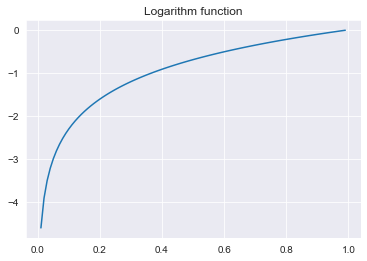
\includegraphics[width=0.8\linewidth]{logarithm.png}
      \caption{Logarithm}
      \label{fig:Logarithm function on (0, 1)}
    \end{minipage}%
    \begin{minipage}{.5\textwidth}
      \centering
      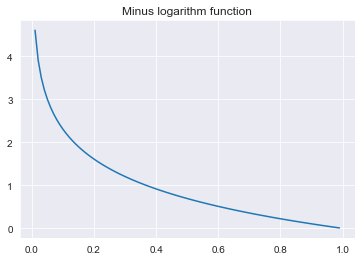
\includegraphics[width=0.8\linewidth]{minlog.png}
      \caption{Minus logarithm}
      \label{fig:Minus logarithm on (0, 1)}
    \end{minipage}
\end{figure}

With this in mind we have:

\begin{enumerate}
    \item $-log(p)$ for $y=1$
    \item $-log(1-p)$ for $y=0$
\end{enumerate}

and cost function $$J = \frac{1}{n}\sum_1^{n}(-y_{i}log(p_{i}) - (1-y_{i})log(1-p_{i})))$$

We can apply the same gradient descent algorithm, as the cost function in this case is convex (this can be proved by checking the sign of the second derivative). 

$$\frac{\partial J}{\partial \beta} = \frac{\partial J}{\partial h} \frac{\partial h}{\partial \beta^{T}x}\frac{\partial \beta^{T}x}{\partial \beta^{T}}$$

$$\sigma(x) = \frac{e^{x}}{1 + e^{x}}$$
$$\sigma(x)' = \sigma(x)(1 - \sigma(x))$$

$$\frac{\partial{J}}{\partial{h}} = -\frac{1}{n}\sum_{1}^n(y_{i}\frac{1}{h(\beta^{t}x)} * \frac{\partial{h}}{\partial{\beta^{T}x}} + (1-y_{i})\frac{1}{1 - h(\beta^{t}x))}\frac{\partial{(1 - h(\beta^{t}x))}}{\beta^{T}x})$$
$$= -\frac{1}{n}\sum_{1}^n(y_{i})\frac{1}{h(\beta^{t}x)}h(\beta^{T}x)(1 - h(\beta^{T}x)x - (1 - y_{i})\frac{1}{1 - h(\beta^{t}x))}h(\beta^{T}x)(1 - h(\beta^{T}x))x)$$
$$= -\frac{1}{n}\sum_{1}^{n}(y_{i}(1 - h(\beta^{T}x))x - (1 - y_{i})h(\beta^{T}x)x)$$
$$= -\frac{1}{n}\sum_{1}^{n}(y_{i} - y_{i}h(\beta^{T}x) - h(\beta^{T}x) + y_{i}h(\beta^{T}x))x$$
$$= -\frac{1}{n}\sum_{1}^{n}(y_{i} - h(\beta^{T}x))x$$

The logistic regression gradient is the same as the linear regression one, with the difference being the sigmoid function.
In matrix notation:
$$\beta = \beta - \frac{1}{n}(h(\beta^{T}X)- Y)X$$

\maketitle

\end{document}\models